\documentclass[a4paper]{article}

\usepackage[UTF8]{ctex}
\usepackage[a4paper,margin=1in]{geometry}
\usepackage{graphicx}
\usepackage{float}
\usepackage{listings}
\usepackage{longtable}
\usepackage{booktabs}
\usepackage{hyperref}
\usepackage{fancyhdr}
\usepackage{lastpage}
\usepackage{color}
\usepackage{indentfirst}        % 首段缩进
\setlength{\parindent}{2em}     % 缩进2字符
\usepackage{zhnumber}           % 中文编号
\usepackage[dvipsnames]{xcolor}
\usepackage{amsmath}
\usepackage{subfigure}

\newcommand{\projname}{数字图像处理|第三章作业}
\newcommand{\reporttitle}{图像增强技术实验}
\newcommand{\stuno}{23336179}
\newcommand{\authorname}{马福泉}
\newcommand{\major}{计算机科学与技术}
\newcommand{\adviser}{骆伟祺}
\newcommand{\startdate}{2025年10月19日}
\newcommand{\labenddate}{2025年10月19日}
\newcommand{\labroom}{B205}

\pagestyle{fancy} % 使用 fancyhdr 风格
\fancyhf{}      % 清空默认的页眉页脚

% 设置页眉
\fancyhead[L]{\kaishu \projname}      % 左侧页眉显示项目名称
\fancyhead[C]{\kaishu \reporttitle}    % 中间页眉显示报告标题
\fancyhead[R]{\kaishu \authorname} % 右侧页眉显示作者姓名

% 设置页脚
\fancyfoot[C]{第 \thepage 页，共 \pageref{LastPage} 页} % 中间页脚显示页码

% 去除页眉页脚与正文之间的分隔线
\renewcommand{\headrulewidth}{0.4pt}
\renewcommand{\footrulewidth}{0pt}

% 设置文档背景颜色
\definecolor{mybgcolor}{RGB}{0, 0, 0} % 定义背景颜色
\definecolor{NavyBlue}{RGB}{0,0,128} % 添加颜色定义

% MATLAB代码样式配置
\lstdefinelanguage{Matlab}{
  keywords={function,if,else,elseif,end,for,while,do,break,return,switch,case,otherwise,try,catch,global,persistent},
  keywordstyle=\color{blue}\bfseries,
  comment=[l]{\%},
  commentstyle=\color{green!50!black},
  string=[s]{'}{'},
  stringstyle=\color{magenta},
  morestring=[s]{"}{"},
  showstringspaces=false,
  numbers=left,
  numberstyle=\tiny\color{gray},
  stepnumber=1,
  numbersep=10pt,
  backgroundcolor=\color{white},
  tabsize=4,
  showspaces=false,
  showstringspaces=false
}

\lstset{
  language=Matlab,
  basicstyle=\ttfamily\footnotesize,
  keywordstyle=\color{NavyBlue}\bfseries,
  commentstyle=\color{gray},
  stringstyle=\color{red},
  showstringspaces=false,
  extendedchars=false, % 关键：不处理中文
  breaklines=true,
  frame=single,
  frameround=tttt,
  framesep=5pt,
  xleftmargin=10pt,
  xrightmargin=10pt
}

\begin{document}

% 封面
\begin{titlepage}
    \centering
    
\includegraphics[width=10cm]{img/SYSULogo.png}

    \vspace{1em}
    \vspace{1em}
    {\Large \kaishu \projname \par}
    \vspace{3em}

    {\fontsize{40pt}{42pt}\kaishu \selectfont \boldmath \reporttitle\par}
    \vspace*{\fill}

    \begin{center}
    {\Large
    \makebox[5em][s]{学号}:\underline{\makebox[15em][c]{\kaishu \stuno}}\\[1em]
    \makebox[5em][s]{姓名}:\underline{\makebox[15em][c]{\kaishu \authorname}}\\[1em]
    \makebox[5em][s]{专业}:\underline{\makebox[15em][c]{\kaishu \major}}\\[1em]
    \makebox[5em][s]{课程教师}:\underline{\makebox[15em][c]{\kaishu \adviser}}\\[1em]
    \makebox[5em][s]{起始日期}:\underline{\makebox[15em][c]{\kaishu \startdate}}\\[1em]
    \makebox[5em][s]{结束日期}:\underline{\makebox[15em][c]{\kaishu \labenddate}}\\[1em]
    \makebox[5em][s]{实验地点}:\underline{\makebox[15em][c]{\kaishu \labroom}}
    }
    \end{center}

    \vspace*{\fill}
\end{titlepage}

% 目录
\tableofcontents
\newpage

\section{实验概述}

本次实验主要实现数字图像处理中的图像增强技术，包括直方图均衡化、拉普拉斯算子锐化和位平面分析。通过编程实现这些基础的图像处理算法，加深对图像增强原理的理解。

\section{编程练习1：直方图均衡化}

\subsection{理论背景}

直方图均衡化是一种通过重新分布图像的灰度级来增强图像对比度的技术。其基本思想是使输出图像的直方图尽可能接近均匀分布，从而改善图像的视觉效果。

直方图均衡化的变换函数为：
\begin{equation}
s = T(r) = (L-1) \sum_{i=0}^{k} p_r(r_i) = \frac{L-1}{MN} \sum_{i=0}^{k} n_i
\end{equation}

其中，$L$是灰度级数，$MN$是图像像素总数，$n_i$是灰度级$i$的像素数量。

\subsection{实验步骤}

\begin{enumerate}
    \item 读取原始图像并转换为灰度图像
    \item 计算原始图像的直方图
    \item 实现直方图均衡化算法
    \item 计算均衡化后图像的直方图
    \item 显示原始图像、增强图像及其直方图
\end{enumerate}

\subsection{Python核心代码片段}
\begin{lstlisting}[language=Python, caption={直方图均衡化主要流程}]
import cv2
import numpy as np

def calculate_histogram(image):
    """计算图像的直方图"""
    hist = np.zeros(256, dtype=np.int32)
    # 统计每个灰度级的像素数量
    for i in range(image.shape[0]):
        for j in range(image.shape[1]):
            hist[image[i, j]] += 1
    return hist

def histogram_equalization(image):
    """
    直方图均衡化主算法
    实现公式: s = T(r) = (L-1) * sum(p_r(r_i)) = (L-1) * CDF(r)
    """
    height, width = image.shape
    total_pixels = height * width
    
    # 步骤1: 计算原始直方图
    hist = calculate_histogram(image)
    
    # 步骤2: 计算累积分布函数(CDF)
    cdf = np.zeros(256)
    cdf[0] = hist[0]
    for i in range(1, 256):
        cdf[i] = cdf[i-1] + hist[i]
    
    # 步骤3: 计算变换函数 T(r) = (L-1) * CDF(r) / (M*N)
    # L=256(灰度级数), M*N=总像素数
    mapping_function = np.round((255 * cdf) / total_pixels).astype(np.uint8)
    
    # 步骤4: 应用变换函数到原图像
    equalized_image = np.zeros_like(image)
    for i in range(height):
        for j in range(width):
            equalized_image[i, j] = mapping_function[image[i, j]]
    
    return equalized_image, mapping_function, hist, cdf
\end{lstlisting}

\subsection{实验结果}

\begin{figure}[H]
    \centering
    \subfigure[原始图像]{
        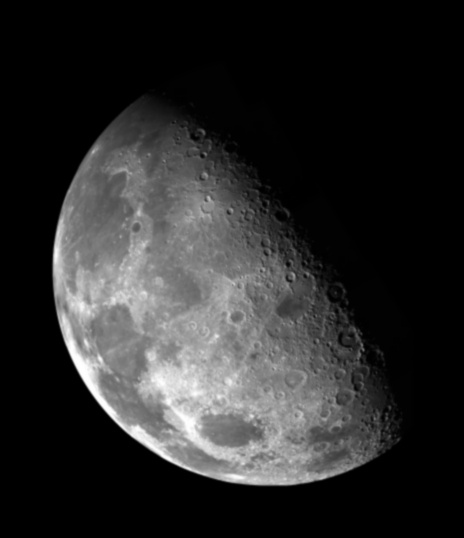
\includegraphics[width=0.4\textwidth]{code/ex1/result/original_image.jpg}
    }
    \subfigure[直方图均衡化后图像]{
        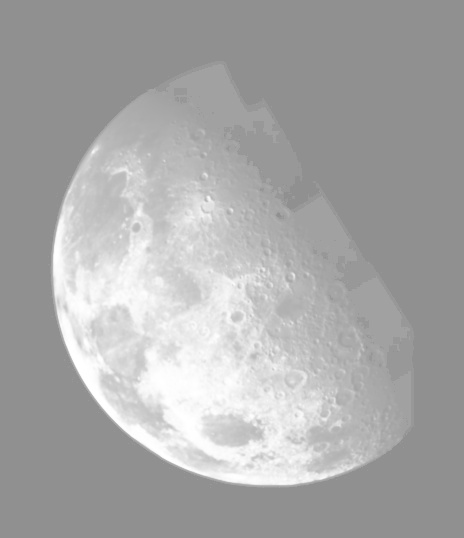
\includegraphics[width=0.4\textwidth]{code/ex1/result/equalized_image.jpg}
    }
    \caption{直方图均衡化结果对比}
\end{figure}

\begin{figure}[H]
    \centering
    \subfigure[原始图像直方图]{
        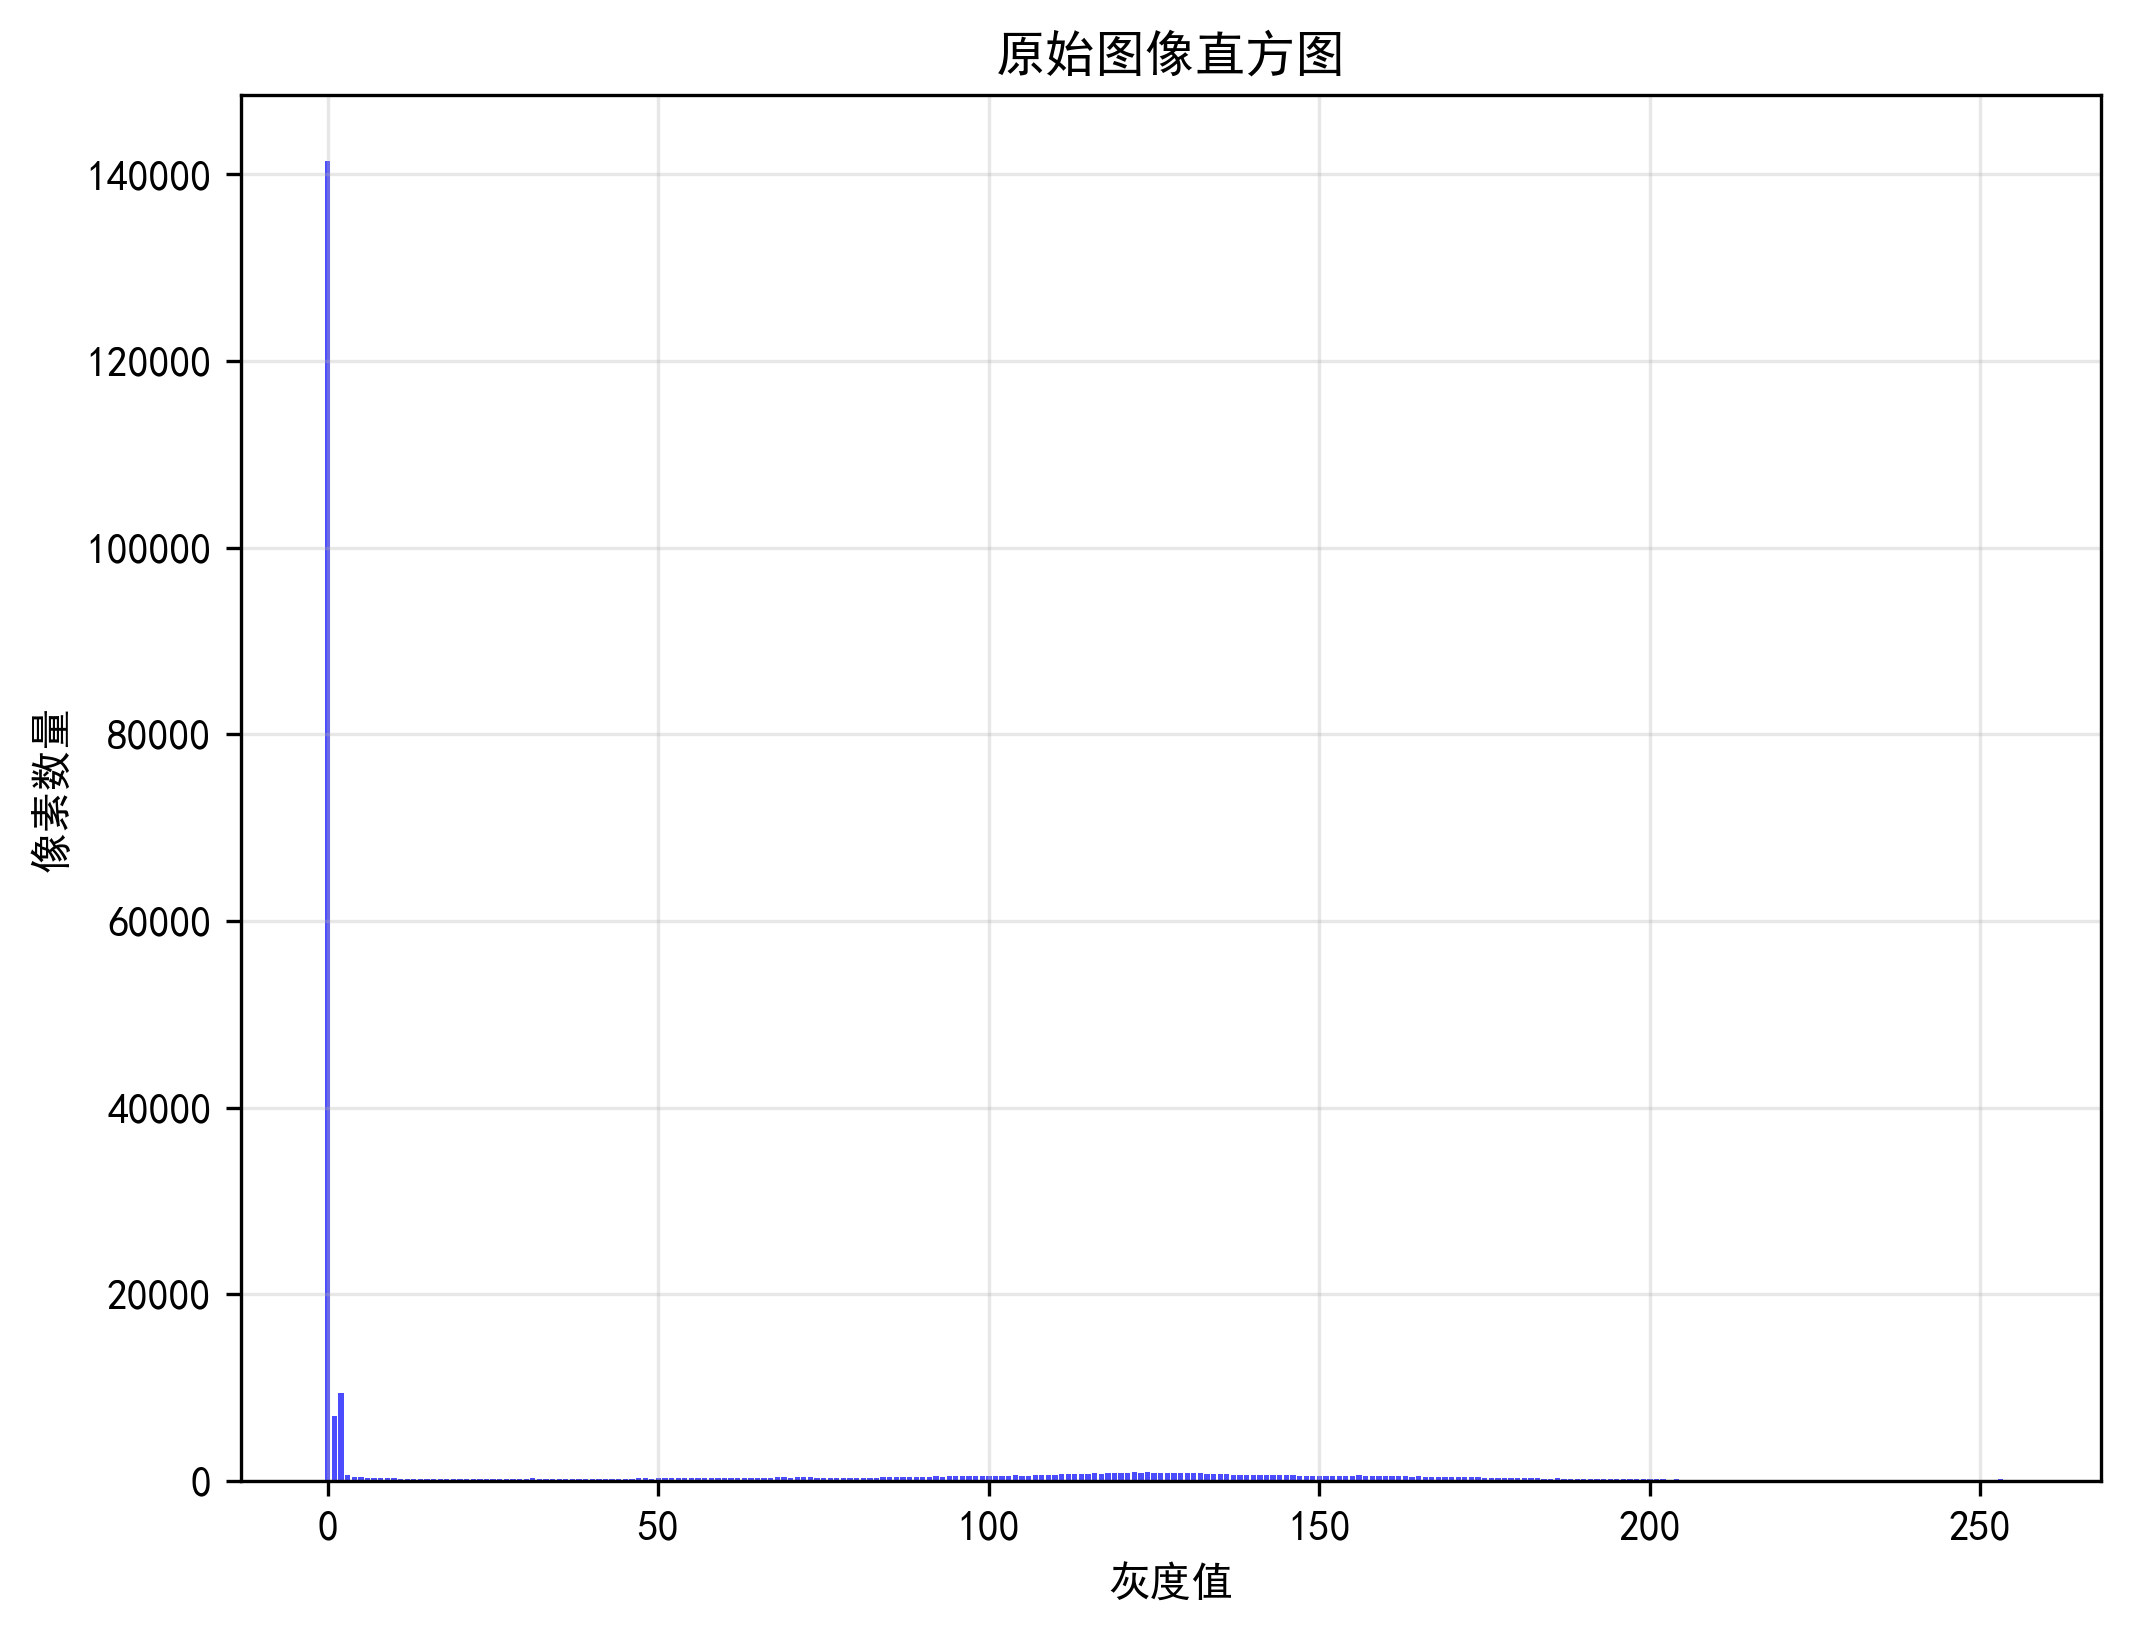
\includegraphics[width=0.4\textwidth]{code/ex1/result/original_histogram.png}
    }
    \subfigure[均衡化后直方图]{
        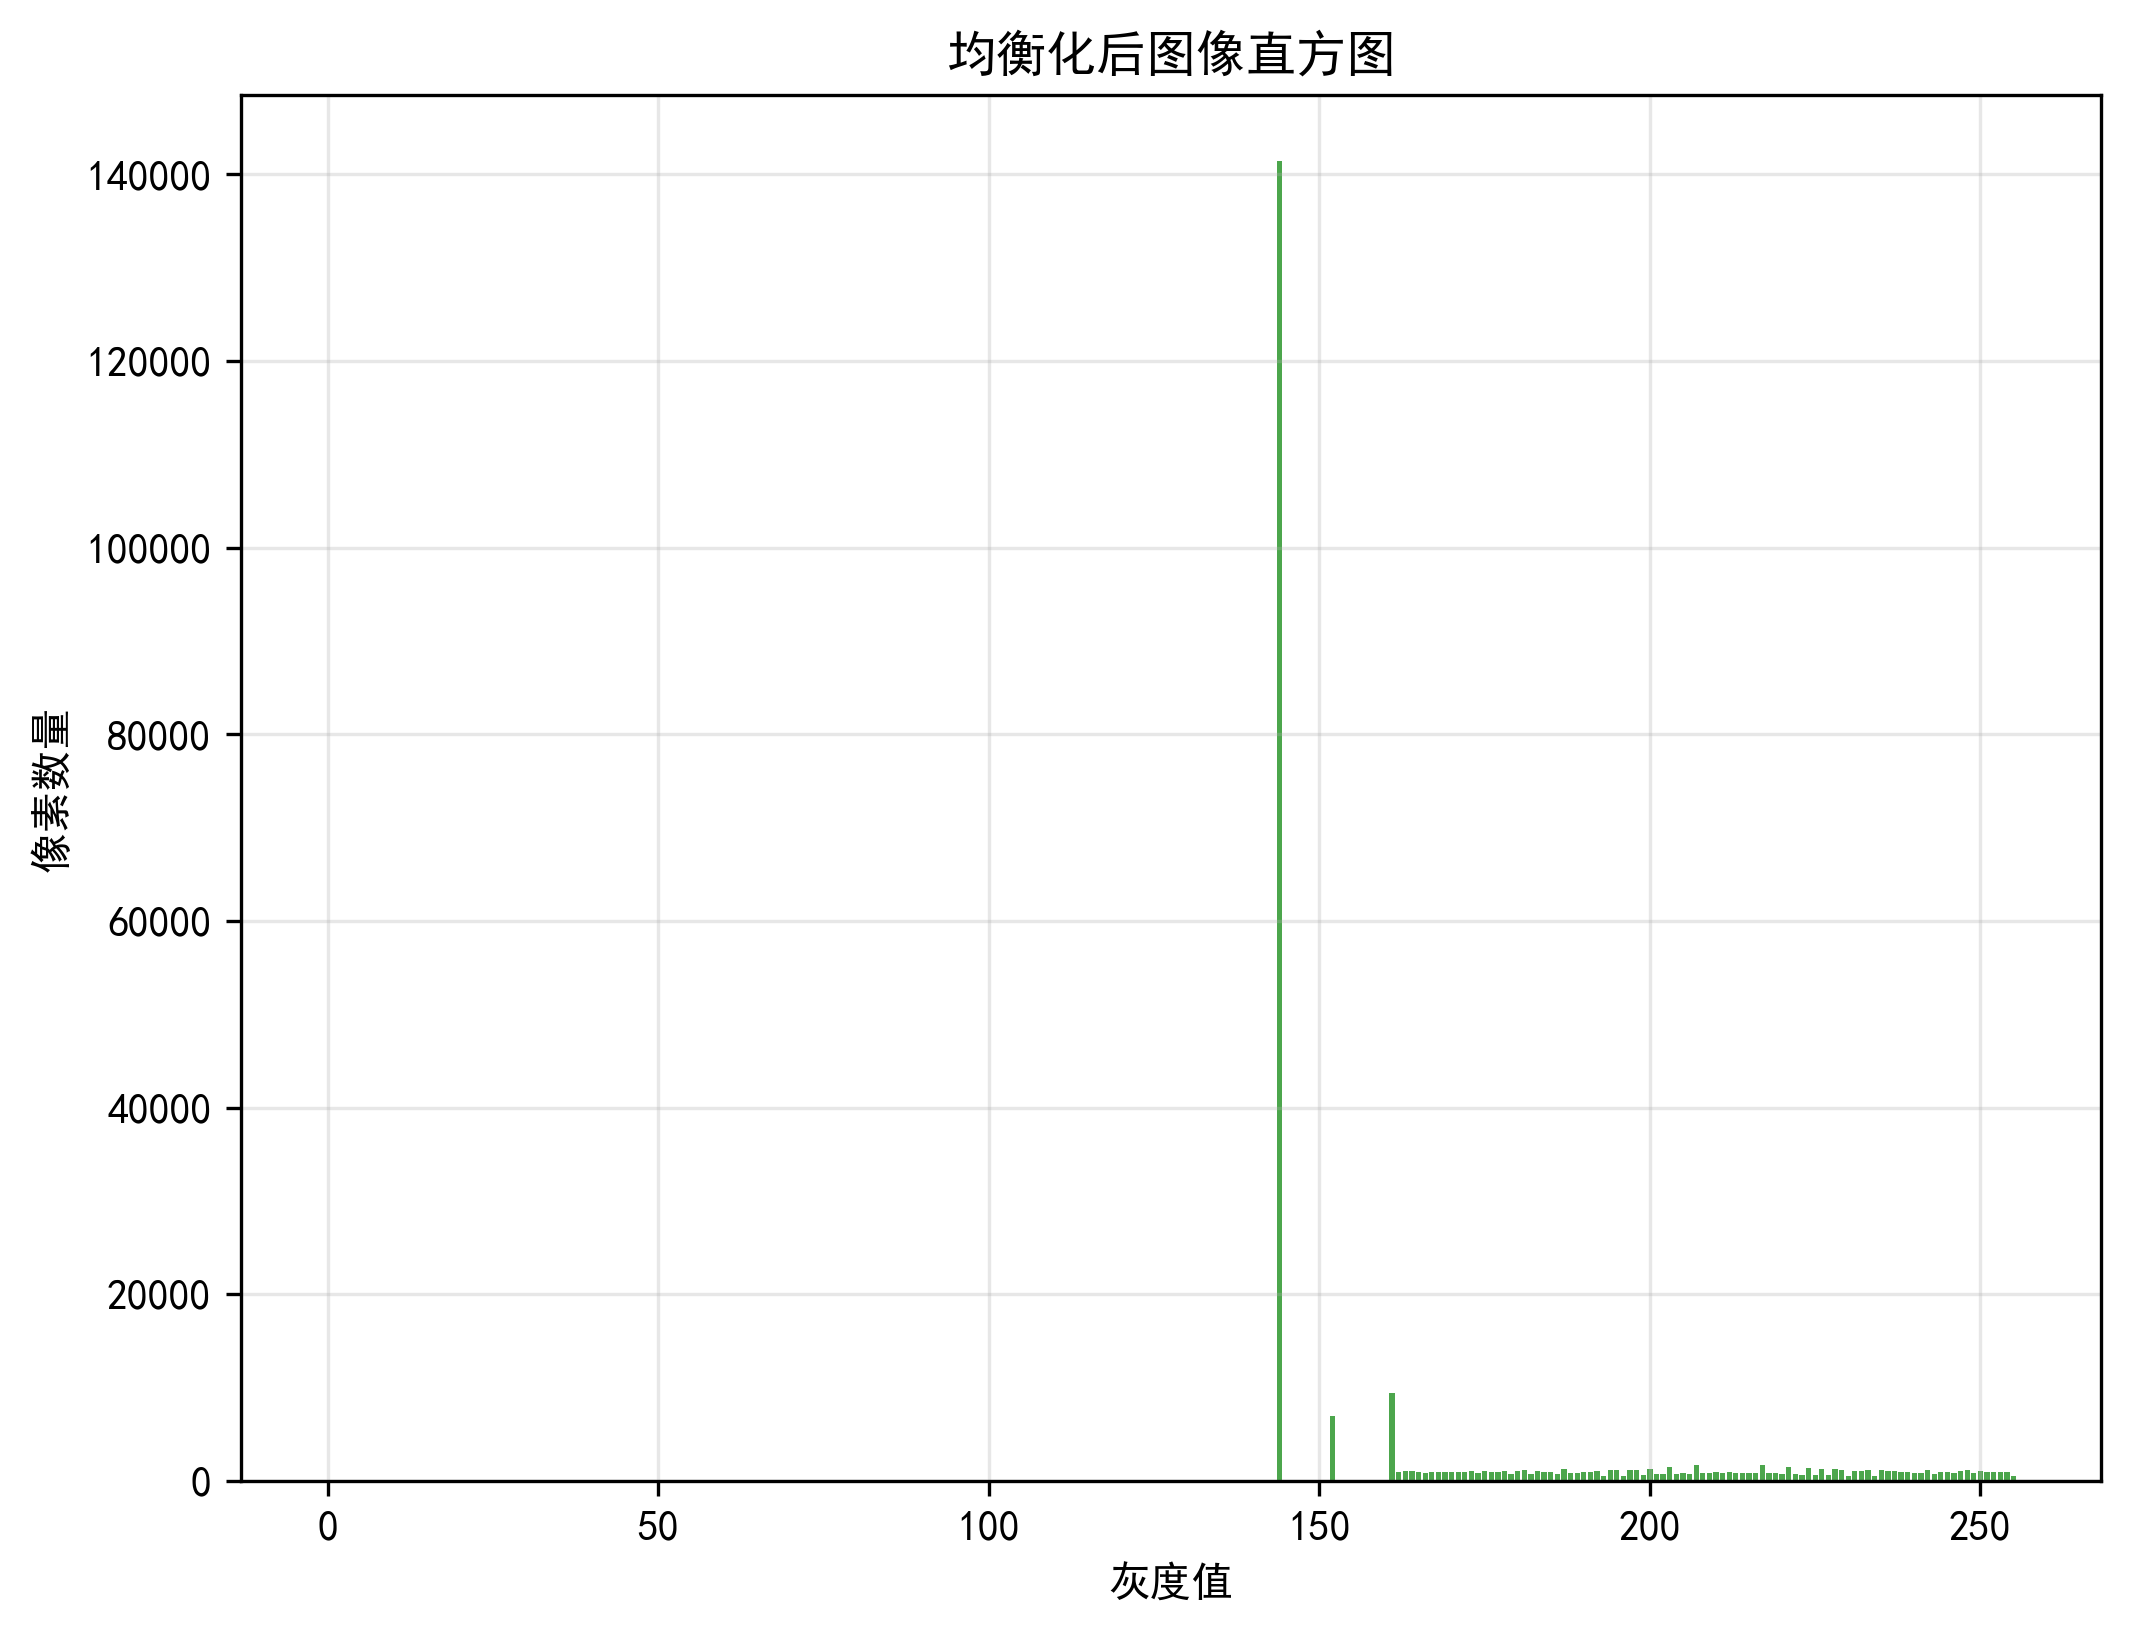
\includegraphics[width=0.4\textwidth]{code/ex1/result/equalized_histogram.png}
    }
    \caption{直方图对比}
\end{figure}

\begin{figure}[H]
    \centering
    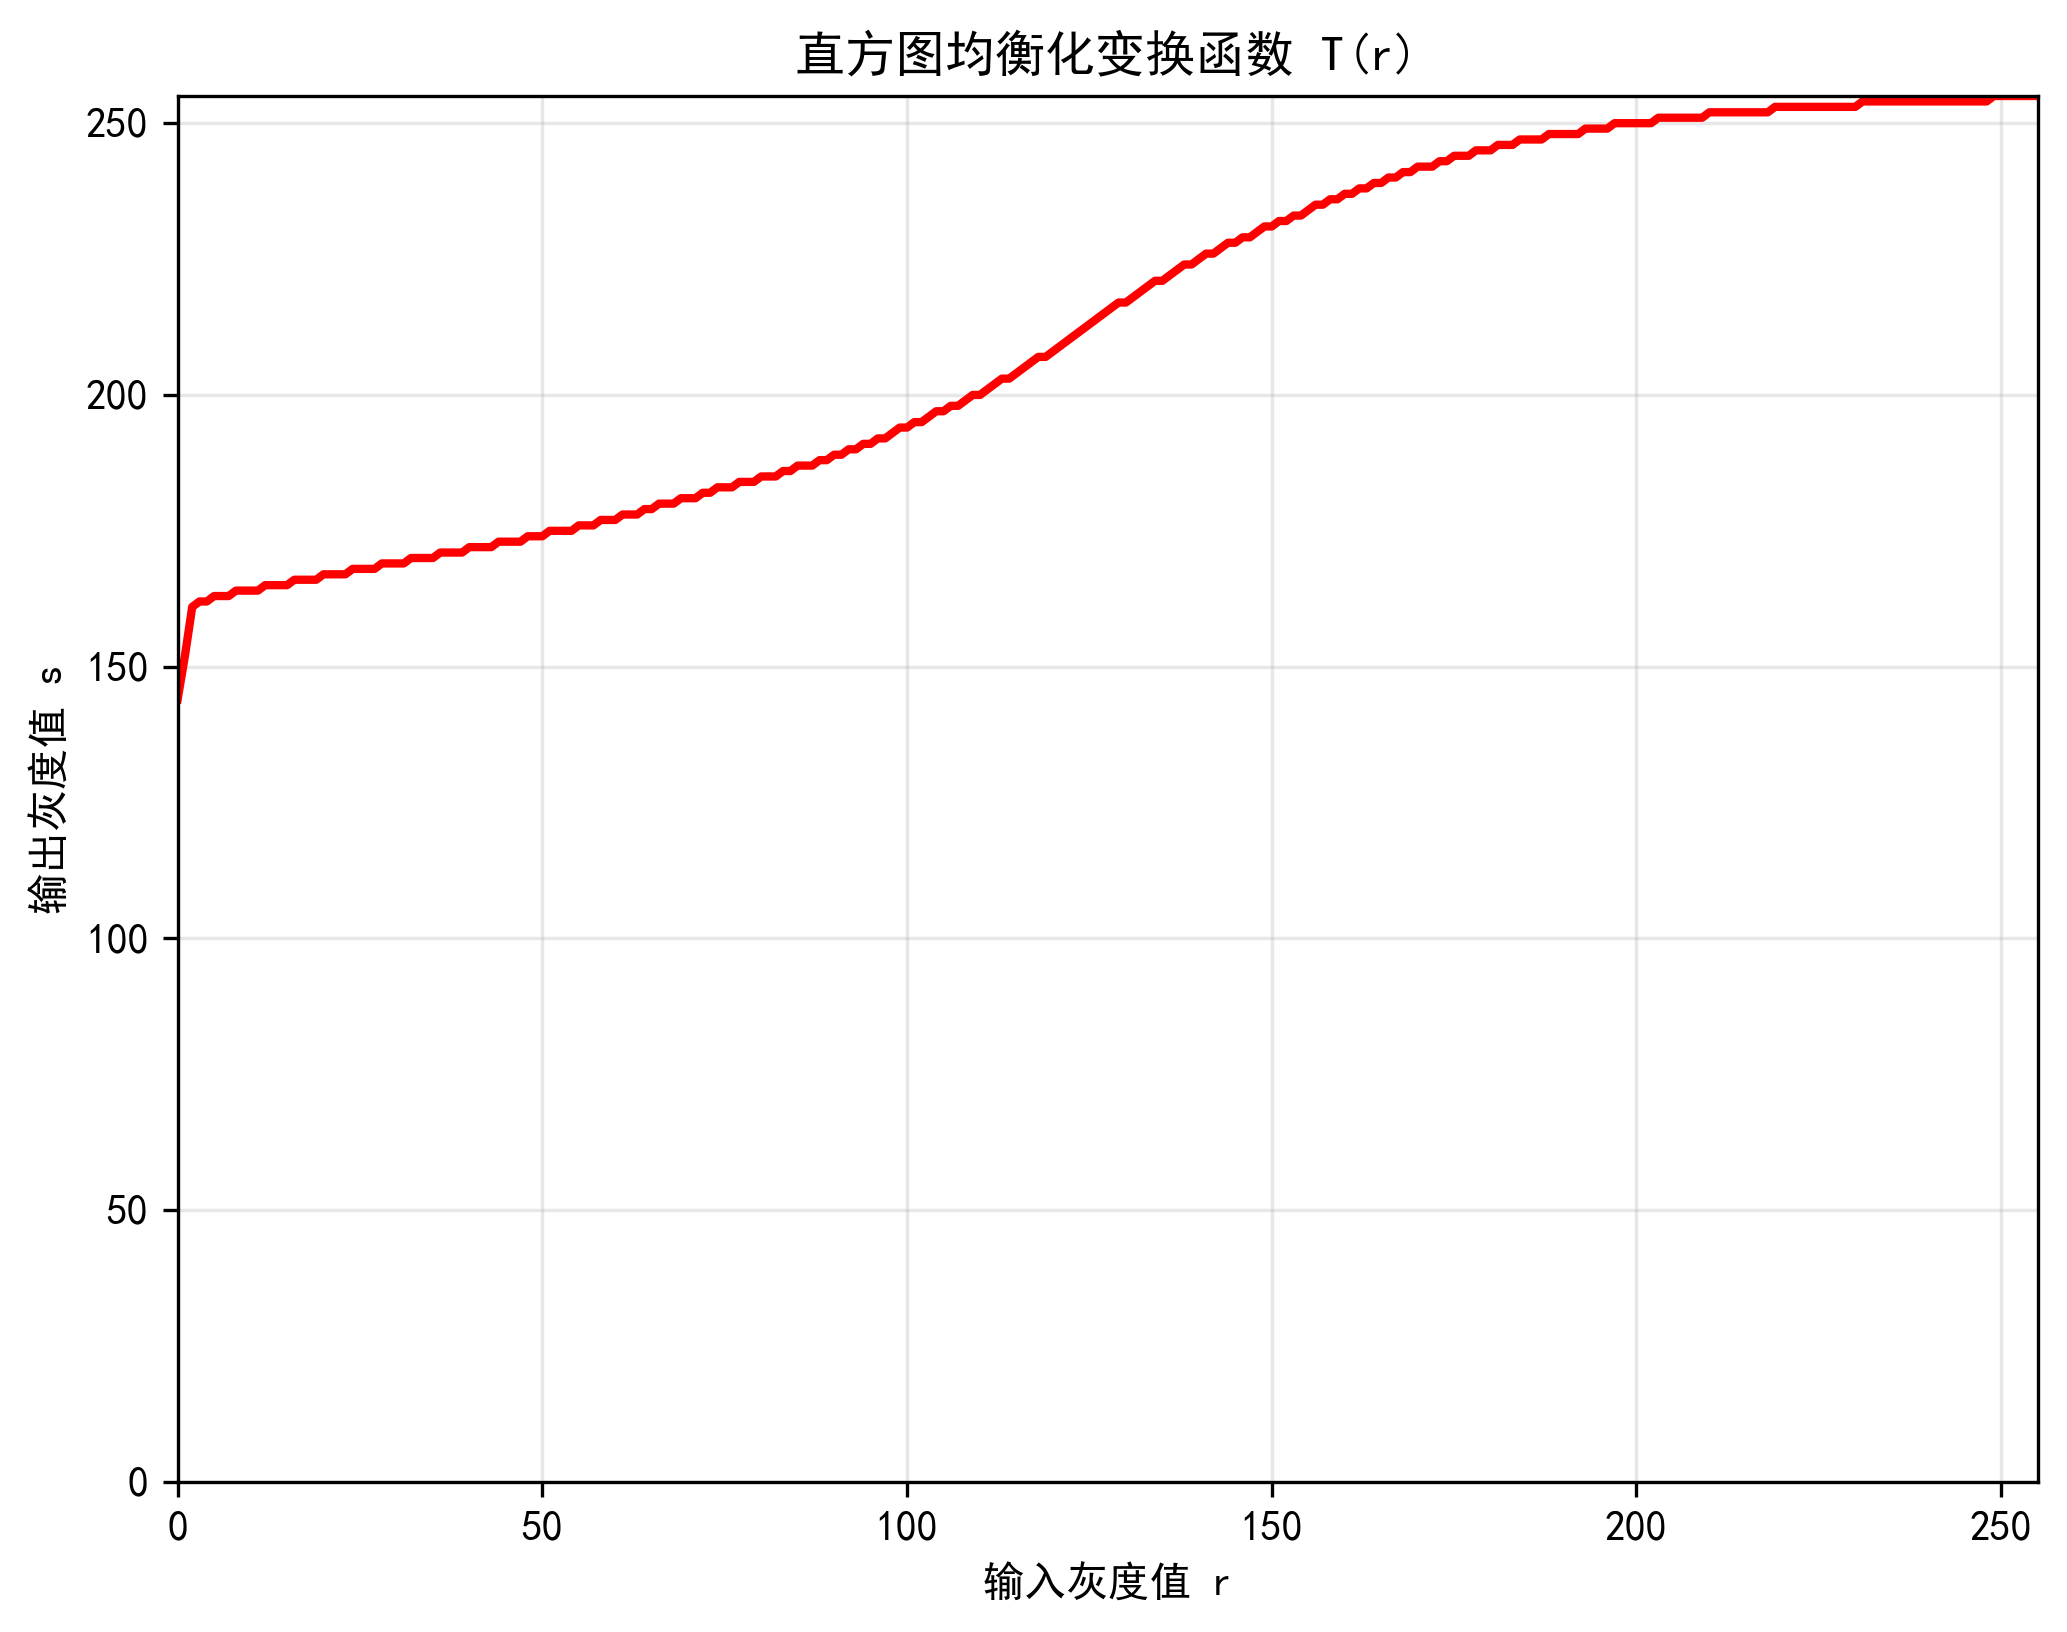
\includegraphics[width=0.6\textwidth]{code/ex1/result/transformation_function.png}
    \caption{直方图均衡化变换函数}
\end{figure}

\subsection{结果分析}

通过直方图均衡化处理，原始图像的对比度得到了显著改善。

\subsubsection{直方图分布特性变化}

\begin{enumerate}
    \item \textbf{原始图像直方图特点}：
    \begin{itemize}
        \item 灰度分布不均匀，主要集中在某些灰度级区间
        \item 存在明显的峰值，表明图像整体偏暗或偏亮
        \item 动态范围利用不充分，导致对比度较低
    \end{itemize}
    
    \item \textbf{均衡化后直方图特点}：
    \begin{itemize}
        \item 灰度分布趋于均匀，各个灰度级的像素数量相对平衡
        \item 充分利用了整个灰度范围[0,255]
        \item 消除了原始直方图的峰值聚集现象
    \end{itemize}
\end{enumerate}

\subsubsection{变换函数分析}

变换函数$T(r)$的特点反映了均衡化的效果：

\begin{itemize}
    \item \textbf{函数形状}：变换函数呈现单调递增的特性，符合理论预期
    \item \textbf{斜率变化}：在原始直方图峰值对应的灰度级处，变换函数斜率较大，表明这些灰度级被"拉伸"
    \item \textbf{映射效果}：低频灰度级被压缩，高频灰度级被扩展，实现了动态范围的重新分配
\end{itemize}

\subsubsection{图像质量改善效果}

\begin{enumerate}
    \item \textbf{对比度增强}：
    \begin{itemize}
        \item 图像的明暗对比更加明显
        \item 细节层次更加丰富
        \item 视觉效果显著改善
    \end{itemize}
    
    \item \textbf{细节信息增强}：
    \begin{itemize}
        \item 原本模糊的细节变得清晰可见
        \item 图像的纹理信息得到突出
        \item 整体视觉质量提升
    \end{itemize}
    
    \item \textbf{动态范围优化}：
    \begin{itemize}
        \item 充分利用了整个灰度空间
        \item 消除了灰度级的浪费现象
        \item 提高了图像的信息容量
    \end{itemize}
\end{enumerate}

\section{编程练习2：拉普拉斯算子增强}

\subsection{理论背景}

拉普拉斯算子是一种二阶微分算子，常用于图像锐化。其离散形式的模板为：
\begin{equation}
\nabla^2 f = \begin{bmatrix}
0 & -1 & 0 \\
-1 & 4 & -1 \\
0 & -1 & 0
\end{bmatrix}
\end{equation}

增强后的图像可以通过以下公式得到：
\begin{equation}
g(x,y) = f(x,y) - c[\nabla^2 f(x,y)]
\end{equation}

其中$c$为增强系数，当$c > 0$时进行锐化。

\subsection{实验步骤}

\begin{enumerate}
    \item 读取原始图像
    \item 定义拉普拉斯核
    \item 对图像进行拉普拉斯滤波
    \item 将滤波结果与原图像相加进行锐化
    \item 显示处理前后的图像对比
\end{enumerate}

\subsection{Python核心代码片段}
\begin{lstlisting}[language=Python, caption={拉普拉斯增强主要流程}]
import cv2
import numpy as np

def manual_convolution(image, kernel):
    """手工实现卷积操作，模拟滤波过程"""
    height, width = image.shape
    k_height, k_width = kernel.shape
    
    # 计算边界填充大小
    pad_h, pad_w = k_height // 2, k_width // 2
    
    # 对图像进行零填充以处理边界
    padded_image = np.pad(image, ((pad_h, pad_h), (pad_w, pad_w)), 
                         mode='constant', constant_values=0)
    
    result = np.zeros_like(image, dtype=np.float64)
    
    # 对每个像素点进行卷积计算
    for i in range(height):
        for j in range(width):
            # 提取与卷积核大小相同的图像区域
            region = padded_image[i:i+k_height, j:j+k_width]
            # 计算卷积值：对应元素相乘后求和
            result[i, j] = np.sum(region * kernel)
    
    return result

def laplacian_enhancement(image):
    """
    拉普拉斯增强算法
    实现公式: g(x,y) = f(x,y) + c*∇²f(x,y)
    """
    # 定义拉普拉斯算子核（8邻域）
    laplacian_kernel = np.array([
        [-1, -1, -1],
        [-1,  8, -1],  # 中心权值为8，周围为-1
        [-1, -1, -1]
    ], dtype=np.float64)
    
    # 计算拉普拉斯响应（二阶微分）
    laplacian_response = manual_convolution(image.astype(np.float64), 
                                          laplacian_kernel)
    
    # 应用增强公式：原图 + 拉普拉斯响应
    enhanced_image = image.astype(np.float64) + laplacian_response
    
    # 限制像素值在有效范围[0,255]内
    enhanced_image = np.clip(enhanced_image, 0, 255)
    
    return enhanced_image.astype(np.uint8), laplacian_response
\end{lstlisting}

\subsection{实验结果}

\begin{figure}[H]
    \centering
    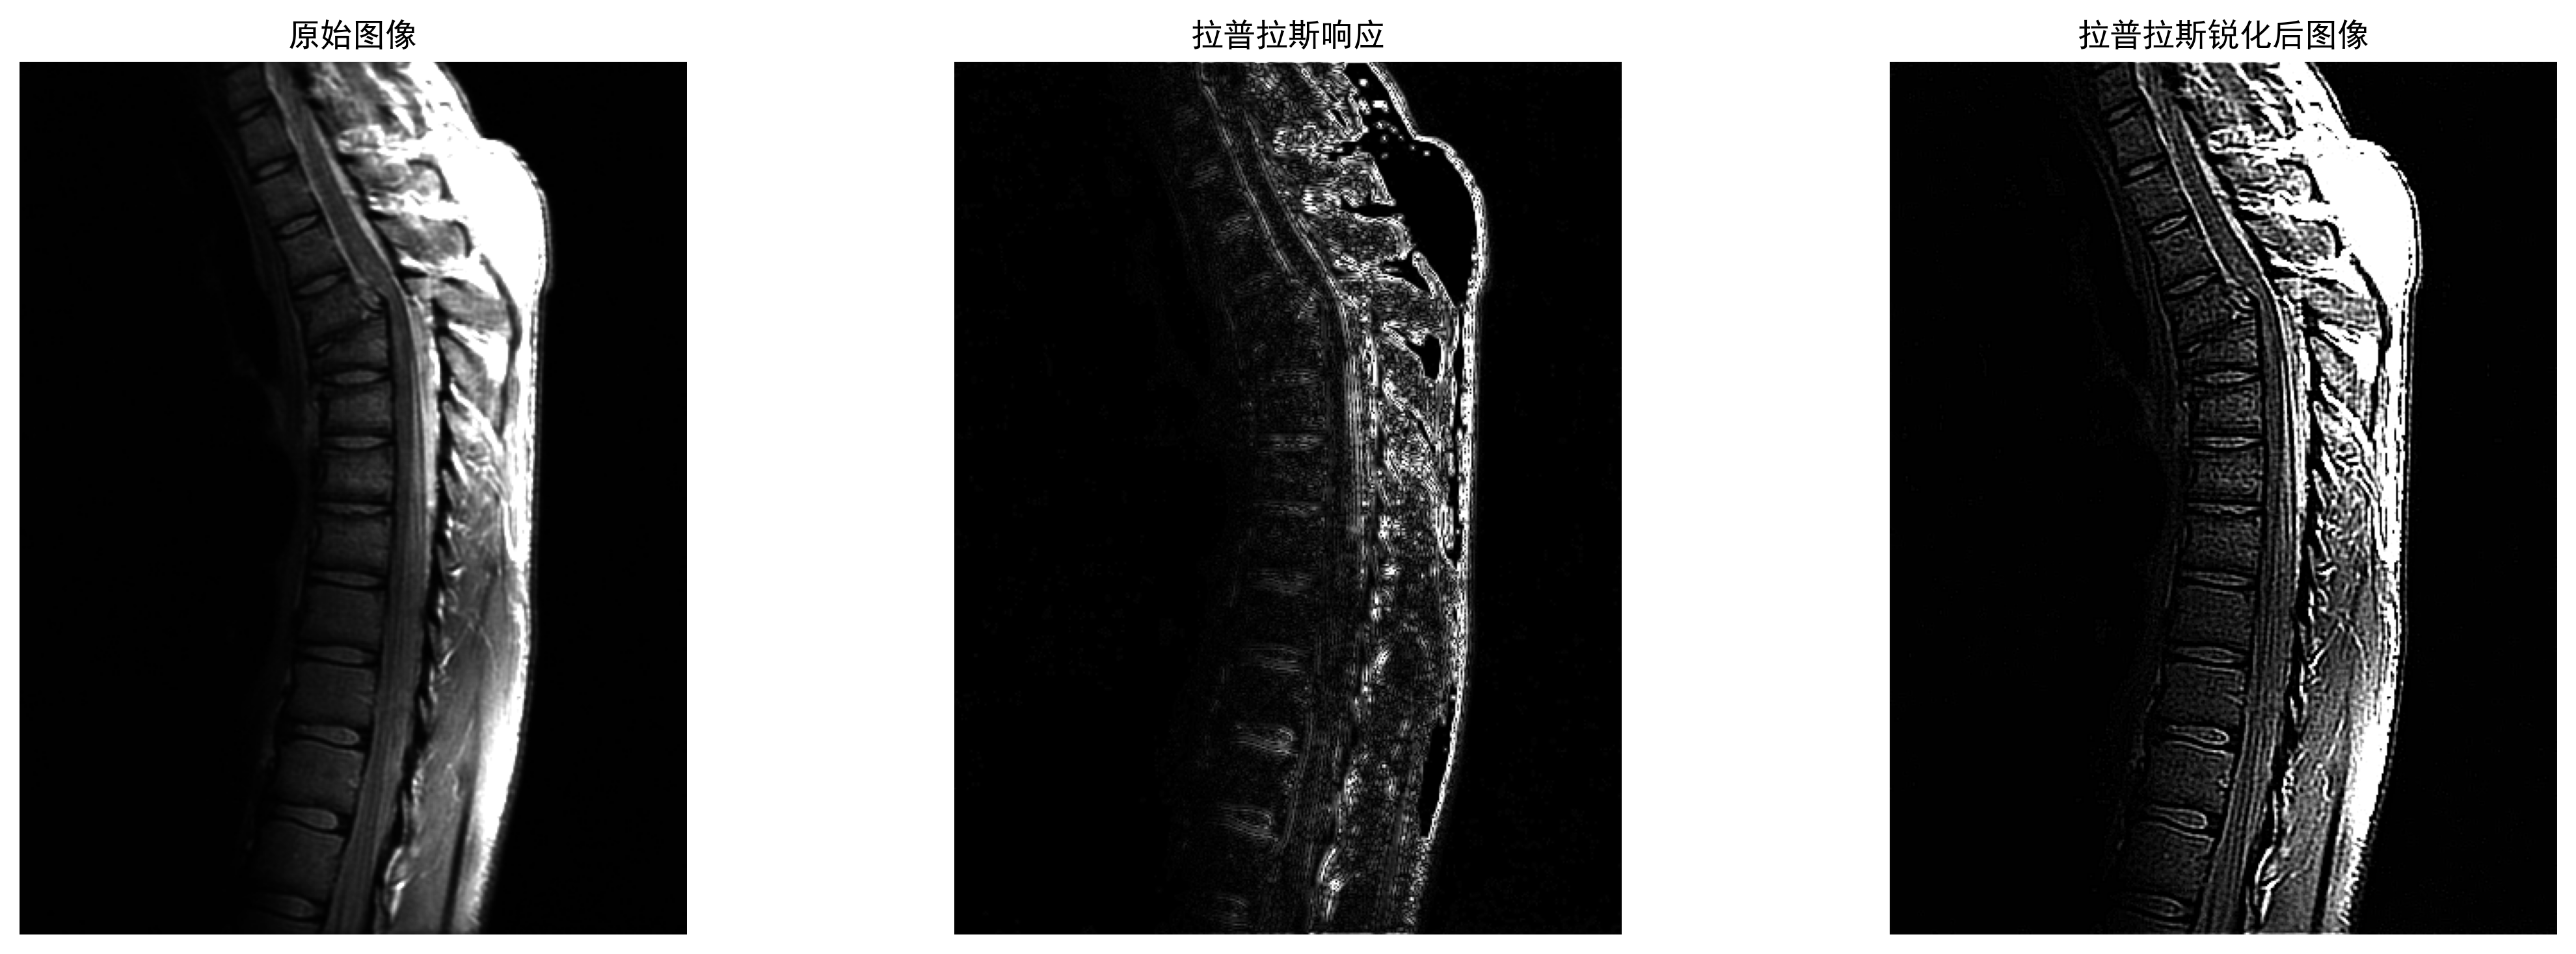
\includegraphics[width=0.9\textwidth]{code/ex2/result/laplacian_enhancement_results.png}
    \caption{拉普拉斯锐化完整结果展示}
\end{figure}

\subsection{结果分析}

拉普拉斯算子成功增强了图像的边缘信息，使图像看起来更加锐利。从结果图中可以看出：
\begin{itemize}
    \item 原始图像经过拉普拉斯滤波后，边缘和细节得到突出
    \item 锐化后的图像边缘更加清晰，细节更加丰富
    \item 拉普拉斯滤波结果显示了图像中的主要边缘结构
\end{itemize}

\section{编程练习3：位平面分析与图像隐写}

\subsection{理论背景}

位平面分析是将图像的每个像素按二进制位分解，得到8个位平面（对于8位图像）。对于一个8位灰度图像，每个像素值可以表示为：

\begin{equation}
I(x,y) = \sum_{i=0}^{7} b_i(x,y) \times 2^i
\end{equation}

其中$b_i(x,y)$表示位置$(x,y)$处像素的第$i$位平面值。高位平面包含图像的主要结构信息，低位平面包含细节信息。最低位平面(LSB)的修改通常不会显著影响人眼的视觉感知，这是图像隐写术的基础。

\subsection{实验步骤}

\begin{enumerate}
    \item 读取灰度图像（使用../img/c.jpg）
    \item 提取8个位平面（从LSB到MSB）
    \item 显示各个位平面的二值图像
    \item 分析各位平面的统计特性
    \item 进行图像隐写实验：使用4种不同模式修改LSB
    \item 计算修改前后图像的差异指标
\end{enumerate}

\subsection{MATLAB核心代码片段}
\begin{lstlisting}[language=Matlab, caption={位平面提取与LSB隐写主要流程}]
function bit_planes = extract_bit_planes(image)
% 提取图像的8个位平面
% 将每个像素的8位二进制表示分解为8个独立的位平面

    bit_planes = cell(8, 1);
    for i = 0:7
        % 右移i位后与1进行按位与操作，提取第i位
        % 例如：像素值170(10101010) >> 1 & 1 = 1
        bit_plane = bitand(bitshift(image, -i), 1);
        % 将0和1映射到0和255便于图像显示
        bit_plane = bit_plane * 255;
        bit_planes{i+1} = uint8(bit_plane);
    end
end

function modified_image = modify_lsb_plane(image, pattern)
% 修改最低位平面进行图像隐写实验
% 实现LSB(Least Significant Bit)隐写技术

    modified_image = image;
    [height, width] = size(image);
    
    switch pattern
        case 'random'
            % 模式1：随机置位，模拟随机信息隐藏
            random_bits = randi([0, 1], height, width, 'uint8');
            % 先清除原最低位(与254按位与)，然后设置新的最低位
            modified_image = bitor(bitand(modified_image, 254), random_bits);
            
        case 'checkerboard'
            % 模式2：棋盘模式，测试规律性模式的影响
            checkerboard = zeros(height, width, 'uint8');
            checkerboard(1:2:end, 1:2:end) = 1;  % 偶数行偶数列设为1
            checkerboard(2:2:end, 2:2:end) = 1;  % 奇数行奇数列设为1
            modified_image = bitor(bitand(modified_image, 254), checkerboard);
            
        case 'zeros'
            % 模式3：全部置0，测试最小修改的影响
            modified_image = bitand(modified_image, 254);  % 清除最低位
            
        case 'ones'
            % 模式4：全部置1，测试最大修改的影响
            modified_image = bitor(modified_image, 1);  % 设置最低位为1
    end
end

function [diff, mse, max_diff] = calculate_difference(img1, img2)
% 计算两幅图像的差异指标
% 用于评估图像隐写的视觉影响

    % 计算像素级绝对差异
    diff = abs(double(img1) - double(img2));
    % 计算均方误差MSE
    mse = mean(diff(:) .^ 2);
    % 计算最大差异值
    max_diff = max(diff(:));
end
\end{lstlisting}

\subsection{实验结果}

\subsubsection{位平面提取结果}

\begin{figure}[H]
    \centering
    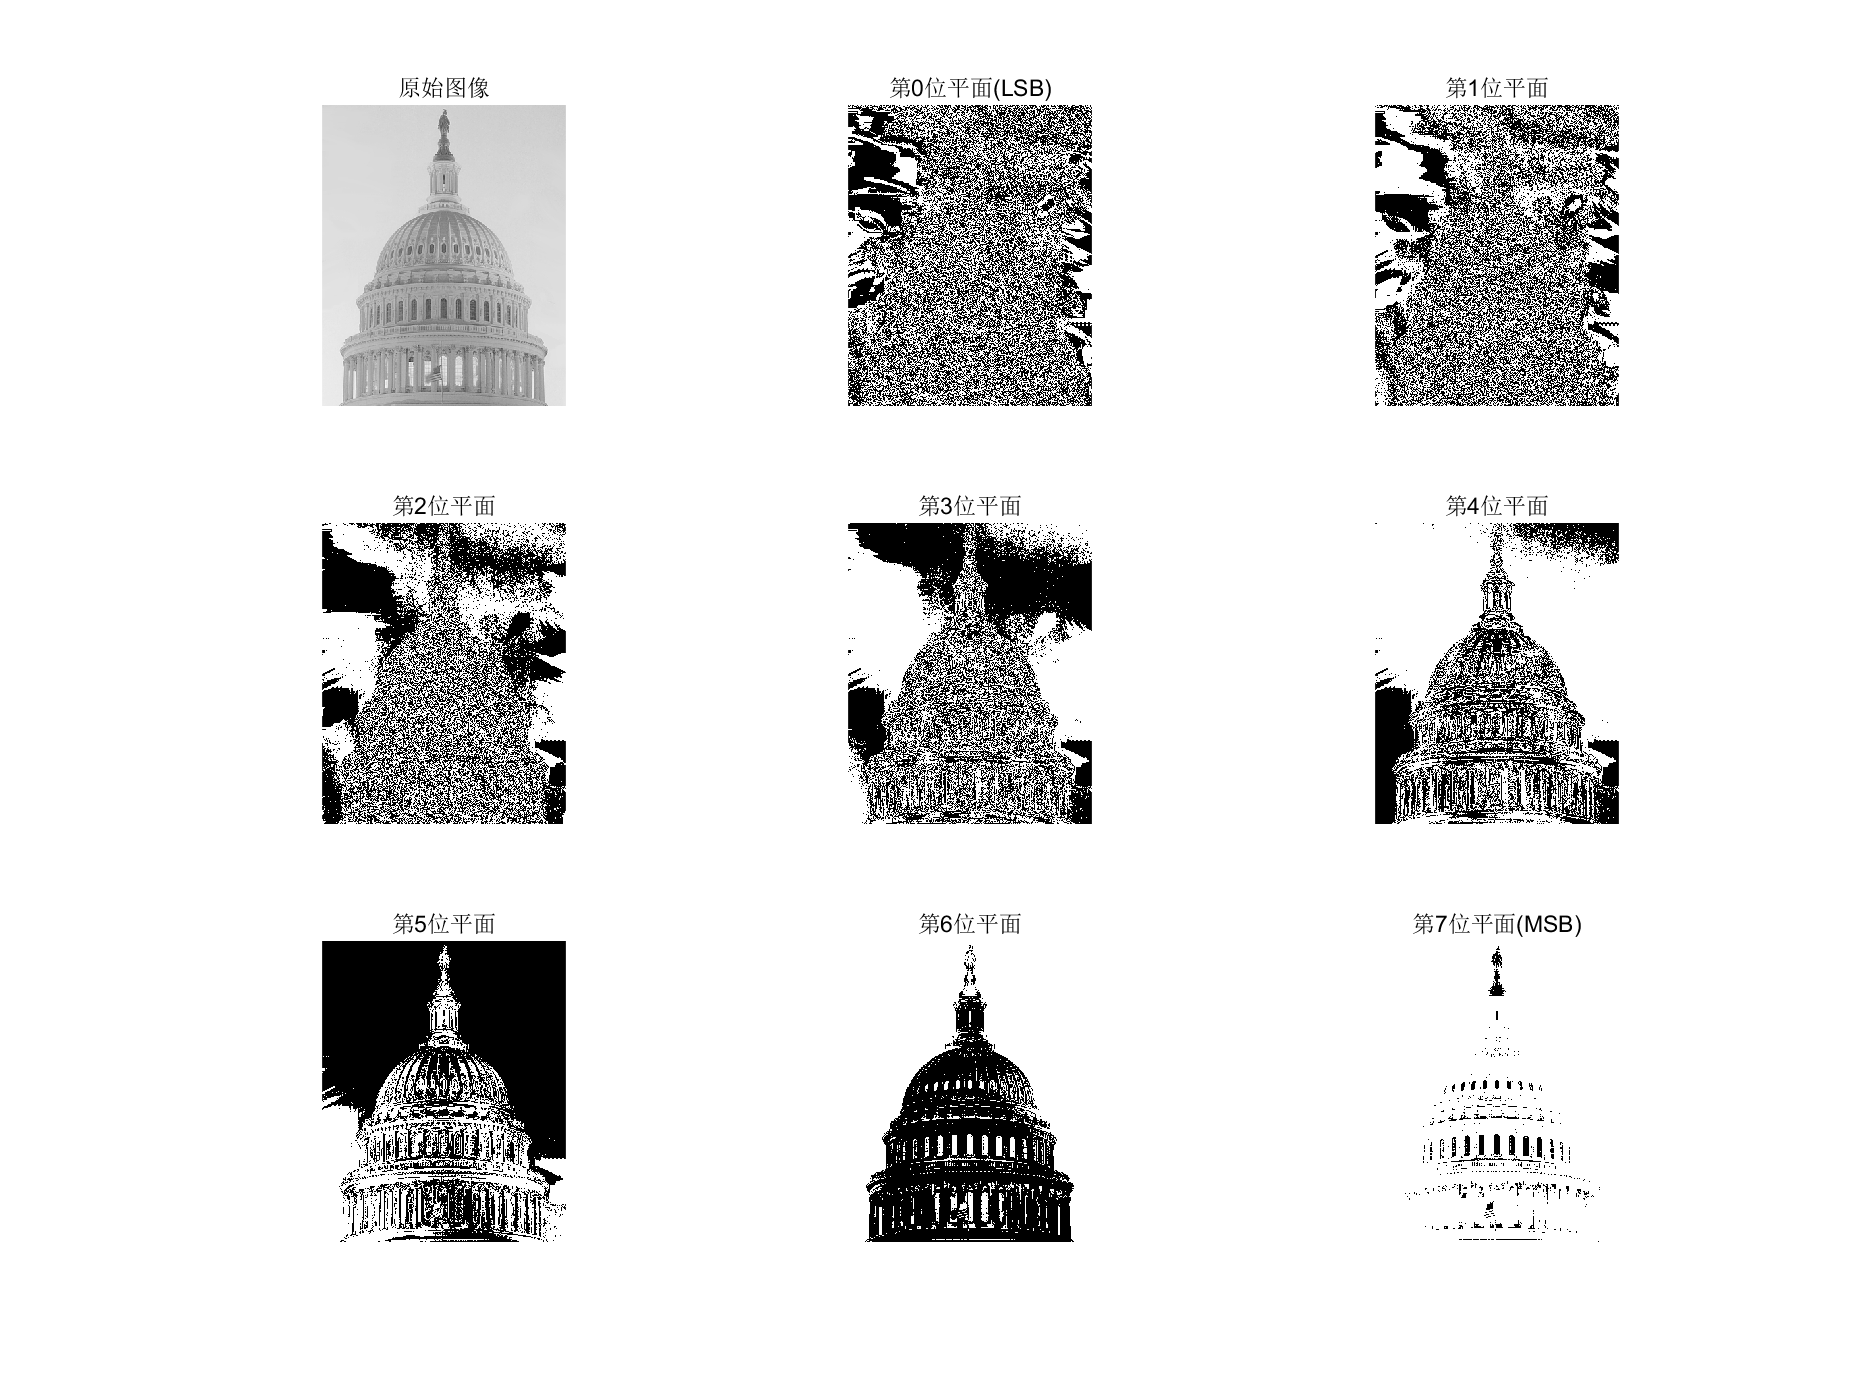
\includegraphics[width=0.9\textwidth]{code/ex3/result/bit_planes_all.png}
    \caption{8个位平面提取结果（从第0位到第7位）}
\end{figure}

\subsubsection{各位平面重要性分析}

通过统计分析，各位平面中像素值为1的比例如表\ref{tab:bit_plane_stats}所示：

\begin{table}[H]
    \centering
    \caption{各位平面统计特性}
    \label{tab:bit_plane_stats}
    \begin{tabular}{|c|c|c|}
        \hline
        位平面 & 描述 & 像素值为1的比例 \\
        \hline
        第0位 & LSB（最低位） & 46.79\% \\
        第1位 & & 50.50\% \\
        第2位 & & 49.96\% \\
        第3位 & & 51.25\% \\
        第4位 & & 65.18\% \\
        第5位 & & 32.26\% \\
        第6位 & & 62.33\% \\
        第7位 & MSB（最高位） & 96.07\% \\
        \hline
    \end{tabular}
\end{table}

从统计结果可以看出：
\begin{itemize}
    \item \textbf{最高位平面（第7位）}：96.07\%的像素为1，包含图像的主要结构信息
    \item \textbf{中高位平面（第6位、第4位）}：分别为62.33\%和65.18\%，包含重要的细节信息
    \item \textbf{低位平面（第0-3位）}：分布相对均匀，接近50\%，主要包含噪声和精细细节
\end{itemize}

\subsubsection{图像隐写实验结果}

对最低位平面进行4种不同模式的修改，实验结果如表\ref{tab:steganography_results}所示：

\begin{table}[H]
    \centering
    \caption{图像隐写实验结果对比}
    \label{tab:steganography_results}
    \begin{tabular}{|c|c|c|c|}
        \hline
        修改模式 & 均方误差(MSE) & 最大差异 & 修改像素比例 \\
        \hline
        Random & 0.500349 & 1.0 & 50.03\% \\
        Checkerboard & 0.499355 & 1.0 & 49.94\% \\
        Zeros & 0.467911 & 1.0 & 46.79\% \\
        Ones & 0.532089 & 1.0 & 53.21\% \\
        \hline
    \end{tabular}
\end{table}

\begin{figure}[H]
    \centering
    \subfigure[Random模式]{
        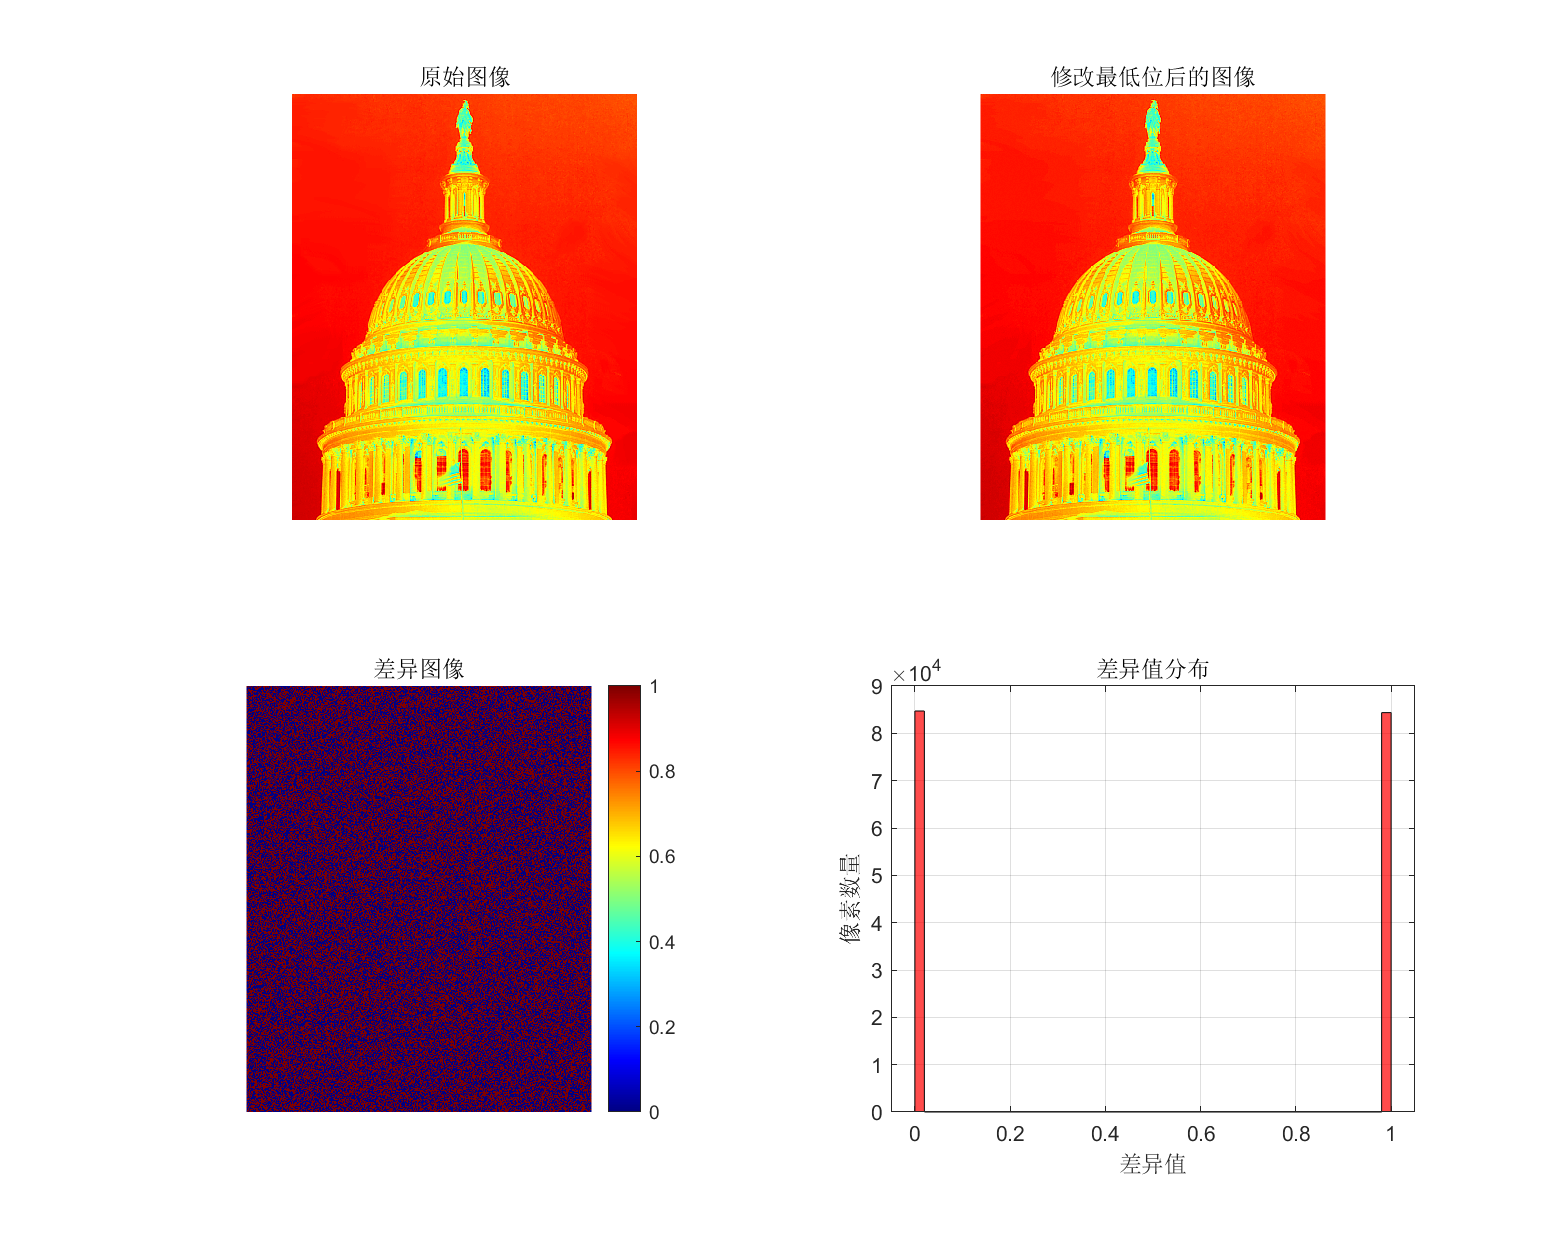
\includegraphics[width=0.45\textwidth]{code/ex3/result/steganography_random.png}
    }
    \subfigure[Checkerboard模式]{
        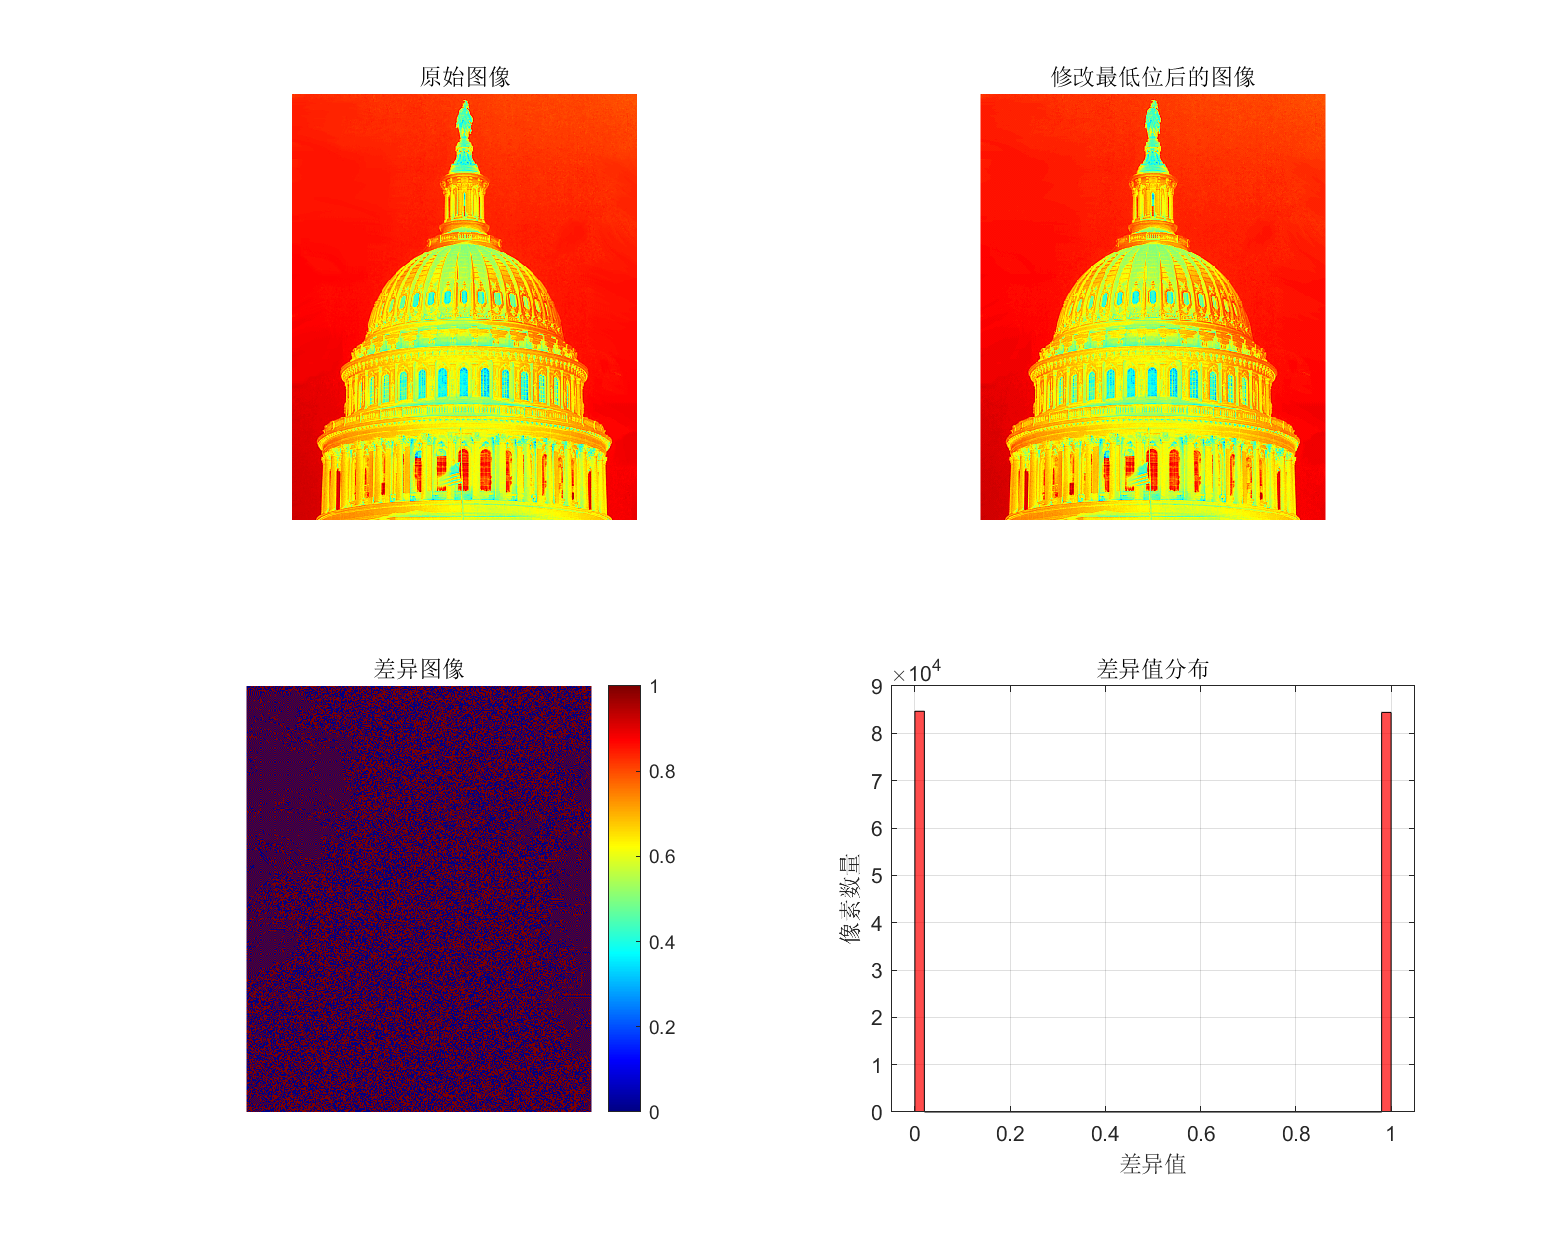
\includegraphics[width=0.45\textwidth]{code/ex3/result/steganography_checkerboard.png}
    }
    \caption{随机模式和棋盘模式隐写对比}
\end{figure}

\begin{figure}[H]
    \centering
    \subfigure[Zeros模式]{
        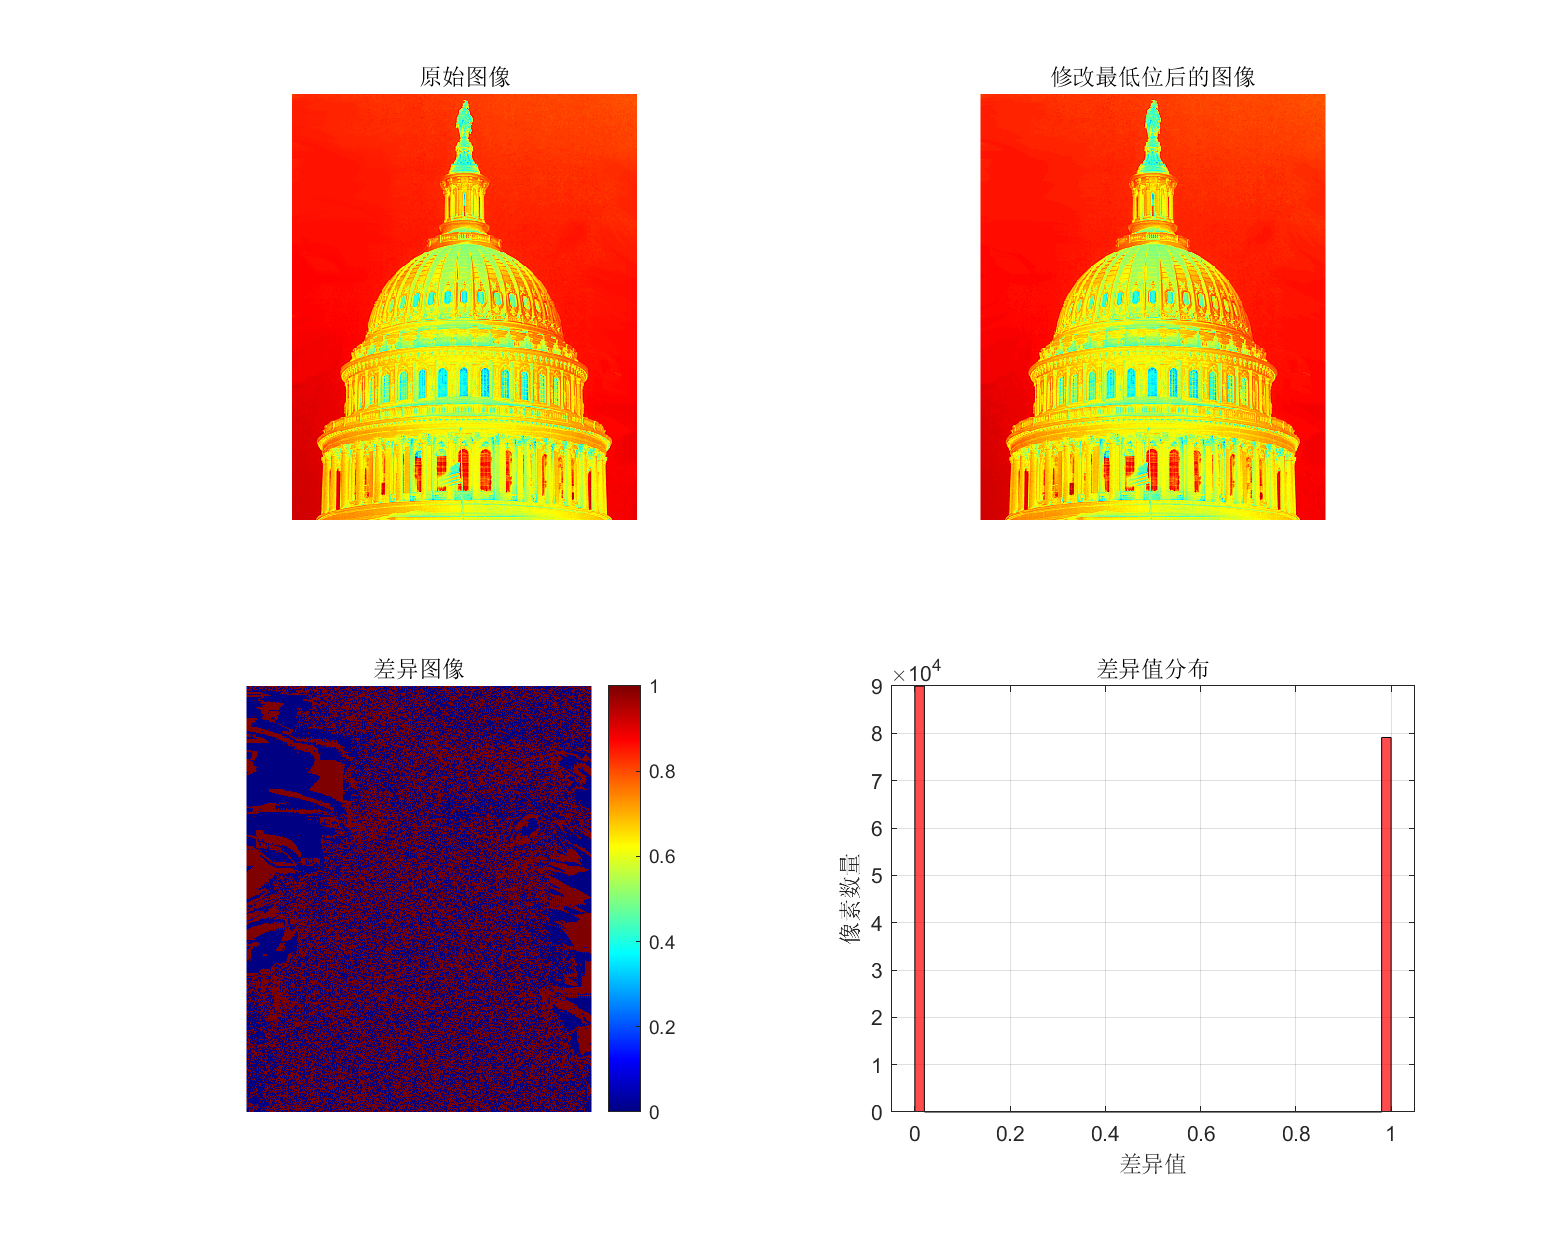
\includegraphics[width=0.45\textwidth]{code/ex3/result/steganography_zeros.png}
    }
    \subfigure[Ones模式]{
        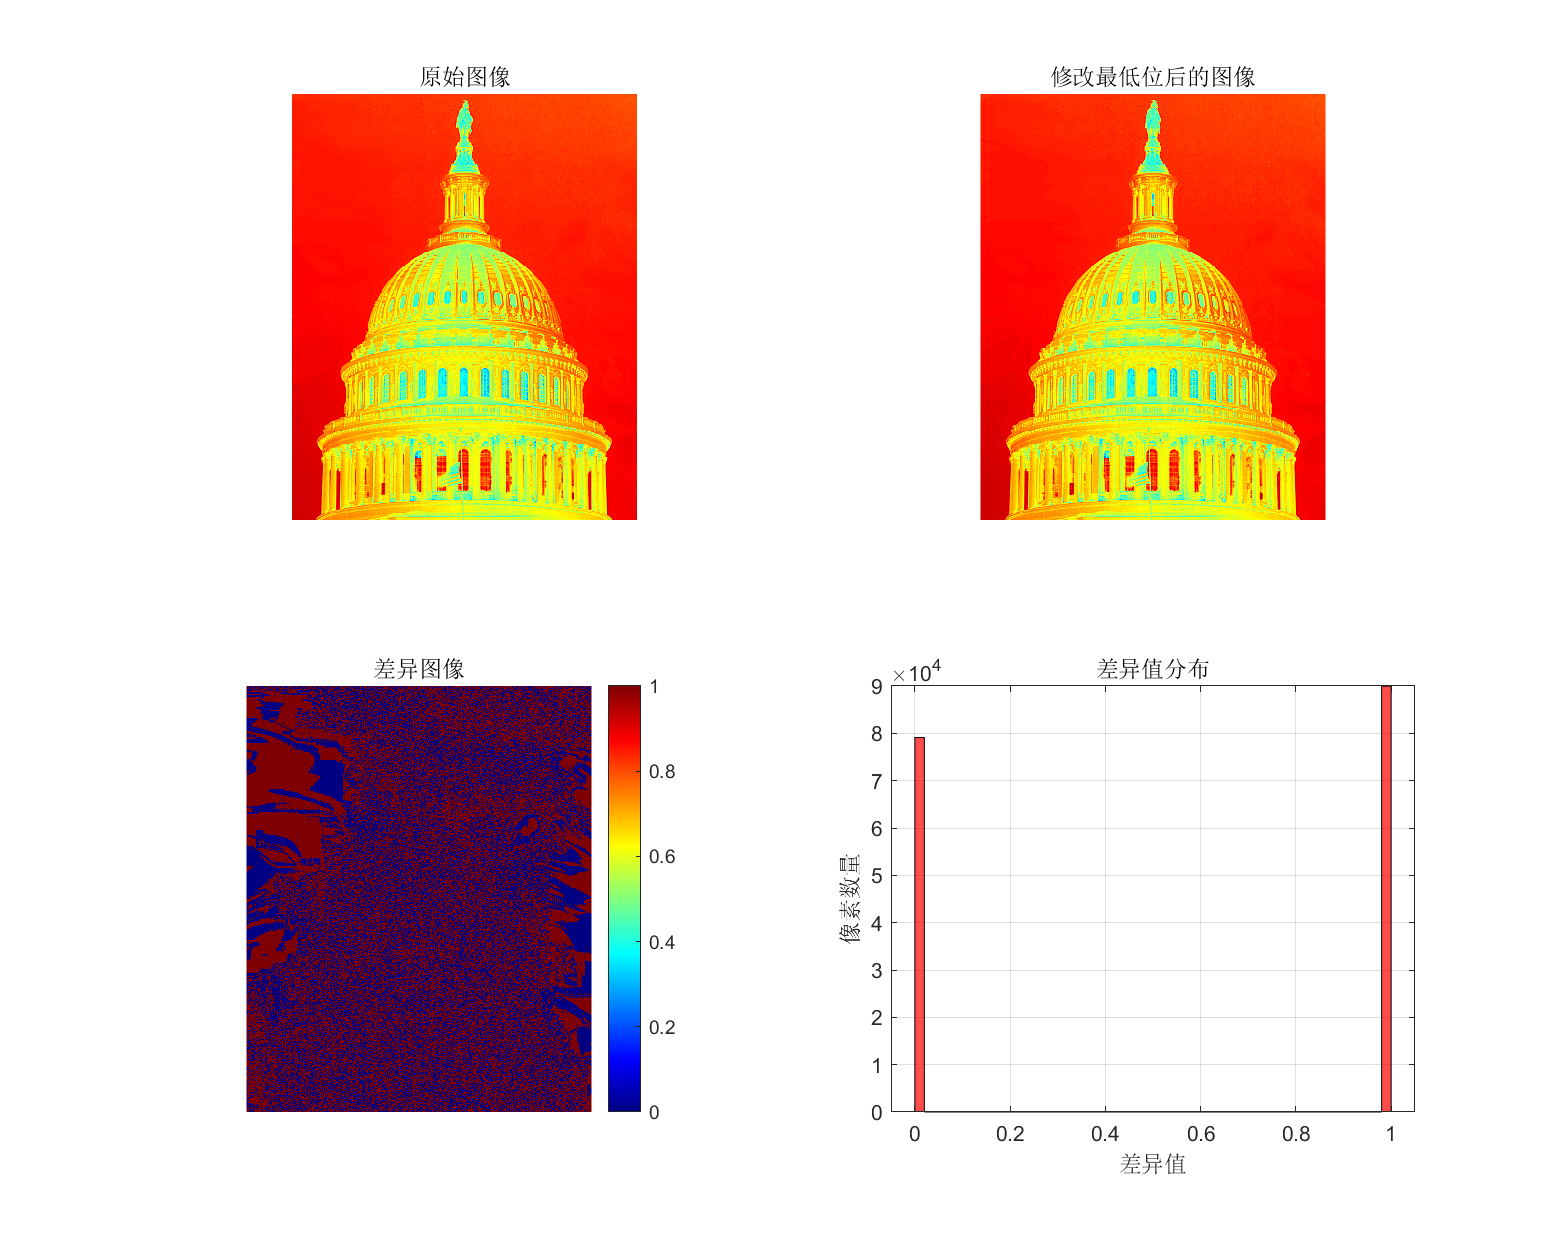
\includegraphics[width=0.45\textwidth]{code/ex3/result/steganography_ones.png}
    }
    \caption{全零模式和全一模式隐写对比}
\end{figure}

\subsection{结果分析}

\subsubsection{位平面特性分析}

从位平面分析结果可以看出：

\begin{enumerate}
    \item \textbf{高位平面重要性}：第7位平面（MSB）包含了图像的主要结构信息，96.07\%的像素为1表明该图像整体较亮
    
    \item \textbf{中位平面细节}：第4-6位平面包含重要的细节信息，其分布反映了图像的纹理特征
    
    \item \textbf{低位平面随机性}：第0-3位平面的分布接近随机，为图像隐写提供了良好的载体
\end{enumerate}

\subsubsection{图像隐写性能评估}

从隐写实验结果分析：

\begin{enumerate}
    \item \textbf{视觉不可感知性}：所有修改模式的最大差异仅为1个灰度级，人眼几乎无法察觉
    
    \item \textbf{统计特性}：
    \begin{itemize}
        \item Zeros模式：MSE最小(0.467911)，因为将LSB全部置0更接近原始分布
        \item Ones模式：MSE最大(0.532089)，将LSB全部置1偏离原始分布较多
        \item Random和Checkerboard模式：MSE约为0.5，表现适中
    \end{itemize}
    
    \item \textbf{隐写容量}：每种模式都能修改约50\%的像素，提供了良好的信息隐藏容量
\end{enumerate}

\subsubsection{图像隐写术理论验证}

实验结果验证了以下重要理论：

\begin{enumerate}
    \item \textbf{LSB隐写可行性}：最低位的修改对图像视觉效果影响极小
    \item \textbf{信息隐藏基础}：为数字水印和秘密通信提供了理论依据
    \item \textbf{安全性考虑}：需要结合密码学方法提高隐写的安全性
\end{enumerate}

\section{实验总结}

本次实验成功实现了三种重要的图像处理技术：

\begin{enumerate}
    \item \textbf{直方图均衡化}：有效改善了图像的对比度，使图像细节更加清晰
    \item \textbf{拉普拉斯锐化}：增强了图像的边缘信息，提高了图像的锐利度
    \item \textbf{位平面分析与图像隐写}：深入分析了图像的位平面特性，验证了LSB隐写的可行性
\end{enumerate}

特别是在位平面分析实验中，通过定量分析各位平面的统计特性和隐写实验，深入理解了：
\begin{itemize}
    \item 图像信息在不同位平面的分布规律
    \item LSB隐写术的理论基础和实际效果
    \item 图像隐写的性能评估方法
\end{itemize}

这些实验为理解图像增强技术原理、图像隐写术和数字水印技术奠定了坚实的基础，为后续更复杂的图像处理算法学习提供了重要的理论和实践支撑。

\end{document}